
\documentclass[]{article}% insert '[draft]' option to show overfull boxes

\usepackage{color}
\usepackage{graphicx,psfrag}
\usepackage{subfigure}
\usepackage{epstopdf}
\usepackage{float}


\usepackage{amssymb}
\usepackage{amsmath}
\usepackage{epstopdf}
\usepackage{morefloats}

\usepackage{graphicx}
\usepackage{amssymb}
\usepackage{appendix}
\usepackage{listings}

%\usepackage{xcolor}
\usepackage{framed}


\lstset{language={[Sharp]c},morecomment=[l]{//} , label=DescriptiveLabel, basicstyle=\ttfamily\scriptsize}
\lstset{frame=shadowbox,}
\lstset{caption=\lstname }


%\usepackage{listings}
%\lstset{
%  language={[Sharp]C},
%  basicstyle=\ttfamily\tiny
%}




\textwidth = 6.5 in \textheight = 9 in \oddsidemargin = 0.0 in
\evensidemargin = 0.0 in \topmargin = 0.0 in \headheight = 0.0 in
\headsep = 0.0 in
\parskip = 0.2in
\parindent = 0.25in

%\newcommand{\comment}[1]{}

%\newtheorem{theorem}{Theorem}
%\newtheorem{corollary}[theorem]{Corollary}
%\newtheorem{definition}{Definition}
%\usepackage{epstopdf
\newcommand{\pd}[2] {\frac{\partial #1}{\partial #2}}
\newcommand{\gfilter}[1] {\overline{#1}}
\newcommand{\tfilter}[1] {\widehat{#1}}
\newcommand{\average}[1] {\langle{#1}\rangle}
\newcommand{\absolute}[1] {\left|{#1}\right|}
\newcommand{\favre}[1] {\widetilde{#1}}

\title{HPC Project: Shade Model Optimization}

\author{Troy Axthelm, Jared Baker, Matthew J. Brazell, Nels Frazier}

\begin{document}

\maketitle
\begin{figure}[H]
\centering
  \begin{tabular}{@{}cccc@{}}
    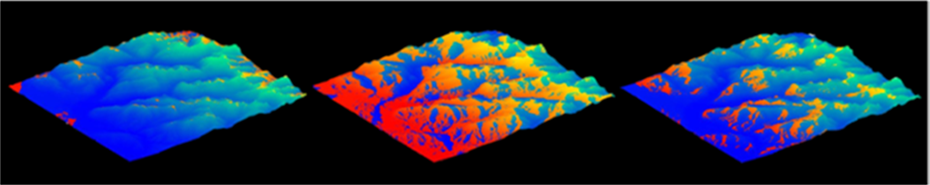
\includegraphics[width=.75\textwidth]{./figures/titleBar.png} 
  \end{tabular}
  \caption{}
  \label{}
\end{figure}

%----------------------------------------------------------------------------------------------------------------------------------------------------------------

%\listoffigures


%----------------------------------------------------------------------------------------------------------------------------------------------------------------
\section{Introduction}

%Talk about the purpose, creaters, and users....

This program is designed to model shade given elevation and location information for a selected land area. With this information a model of watershed can be created for primary use by CI-Water Project for predicting locations for forest fire remediation. The uploaded land area of interest can simply be downloaded off of GIS, the user can select a time interval over the course of a specific day of the year. The GPS coordinates of the land area as well as day of the year provide solar angle along with the topography of the land indicate if an area is shaded or not. Currently the program  only indicates if an element of the land area is shaded or not shaded. No information of temperature or partial shading is provided and may be a future goal however currently this information alone is sufficient for CI-Water Project's needs.

The original program was created by Troy Axthelm and Jingyu Li  funded by CI-Water Project. For more information and location of the open source code please see the link below:

https://sites.google.com/site/uwyoshademodel/

As a project for a graduate coarse: Designing and Building Applications for Extreme Scale Systems lead by instructor William Gropp and Professor Craig Douglas, our group intends make improvements in performance leading to faster simulations as well as making the program more flexible and easier to use for the user during runtime as well as post processing and visualization.

%----------------------------------------------------------------------------------------------------------------------------------------------------------------
\subsection{Initial Benchmarking}

%----------------------------------------------------------------------------------------------------------------------------------------------------------------
\subsubsection{Parlib MPI}

To test functionality of different Message Passing Interface (MPI) routines and avoid conflicts with Parlib, we decided to remove the Parlib dependency in this particular case. While there are advantages to having an interface library, we are exploring different methods with MPI which are not yet implemented in Parlib, such as MPI derived data types and structures. To effectively pass structures in MPI as an array data type, we needed to utilize a method which was not available in the Parlib implementation. This was a primary driving factor for removing the interface code in this particular case. There was also possibility that we may have implemented MPI-3 routines which were not also available in the Parlib implementation.
%----------------------------------------------------------------------------------------------------------------------------------------------------------------
\subsubsection{MPI}

An initial profiling of the code in parallel was used to determine trouble areas in the code where performance improvements could be made. The result of using the Allinea profiler showed that over 80\% of the computing time was spent in a loop in main.c, the specific code for this problem area is shown below for convienence:
{\small
\begin{verbatim}

//Step along azimuth until off of grid or the observer point is determined to be shaded
while (tempX >= 0 && tempX <= (numCols-1) && tempY >= 0 && tempY <= (numRows - 1))
{	

	roundTempX = (int)round(tempX);
	roundTempY = (int)round(tempY);			

	if(roundTempX != i ||  roundTempY != j) 
	{
		tempSlope = (ourData[roundTempY][roundTempX].elevation - ourData[i][j].elevation)/sqrt(lenX*lenX + lenY*lenY);	

		if(solarAlt <= tempSlope)
		{	
			ourData[i][j].shading[k] = 1;
			break;
		}
	}												

	lenX += stepX;		
	lenY += stepY;

	tempX += stepTempX;
	tempY += stepTempY;

}
\end{verbatim}}


%----------------------------------------------------------------------------------------------------------------------------------------------------------------
\subsection{Performance Model}

A performance model was created to give us a rough idea on the expected timing in the area described above where over 80\% of the computation time is spent. The model is defined as:

total time $=n*m*(8r+5w+2c)$

assuming the time for write is equal to the time for read then:

total time $=8 (\frac{bytes}{element})*n*m*(13*r*\frac{1Mbytes}{1e6 bytes} + 2c)$

with n=1966 and m=2054, using the Stream performance the best Rate shown in table \ref{table:STREAM} an estimate for the performance of a read is 15564.0 MB/s, time for a read is $\frac{1}{15564.0 MB/s}$


The compute nodes on Mt. Moran used for testing use Intel chips with 2.6 GHz which gives an estimate of $c=2.6e9$ flops. The estimated time based on this performance model gives t=$  0.09159 $seconds if we assume 1-4 bytes moved per 32 bytes for each floating point operation gives 0.96\% to 3.8\% of peak performance giving an estimated time  of t=$8.7926e-4$ to  t=$0.0035$ [Sec]

\begin{table}[ht]
\caption{Stream Results on Mt. Moran}
\centering
\begin{tabular}{c c  c c c}
\hline\hline
\hline
Function   & Best Rate MB/s & Avg time  &   Min time &    Max time \\ [0.5ex] 
\hline

Copy:    &     14078.4    & 0.011393    & 0.011365     & 0.011444\\
Scale     &  14098.2    & 0.011366     & 0.011349    & 0.011390\\
Add:      & 15564.0    & 0.015445     & 0.015420     & 0.015477\\
Triad:    & 15379.7    & 0.015635     & 0.015605     & 0.015659\\

\hline
\end{tabular}
\label{table:STREAM}
\end{table} 


%----------------------------------------------------------------------------------------------------------------------------------------------------------------
\subsection{Coding Improvements}

%----------------------------------------------------------------------------------------------------------------------------------------------------------------
\subsubsection{Algorithmic Improvements}
introduce global constants
reduce built in algebraic functions
example code from landReader.c:

$temp.latitude = latitude*180.0/(4*atan(1))$;	$//convert the latitude to degrees	$

where $4*atan(1) = 3.141592653589793 = \pi$

%----------------------------------------------------------------------------------------------------------------------------------------------------------------
\subsubsection{Linear Memory}

To make improvements to the part of the code where the majority of the compute time is taken, by improving the way the array's "outData.elevation" is read and "ourData.shading" is written will make significant improvements to performance. To verify that this is an area that can be improved a simple performance model is created and compared with timing results of the actual code over this loop. This performance model is only to demonstrate an upper limit on performance.

{\small
\begin{verbatim}

									//Step along azimuth until off of grid or the observer point is determined to be shaded
loop through numCols & numRows: n,m		while (tempX >= 0 && tempX <= (numCols-1) && tempY >= 0 && tempY <= (numRows - 1))
									{	
									
%n*m*(r+0.5*w)								roundTempX = (int)round(tempX);
%n*m*(r+0.5*w)								roundTempY = (int)round(tempY);			
									
										if(roundTempX != i ||  roundTempY != j) 
										{
n*m*((2+4*0.5)*r+w+2c)							tempSlope = (ourData[roundTempY][roundTempX].elevation - ourData[i][j].elevation)/sqrt(lenX*lenX + lenY*lenY);	
									
											if(solarAlt <= tempSlope)
											{	
%n*m*(w)											ourData[i][j].shading[k] = 1;
												break;
											}
										}												
									
%4*n*m*0.5*(r+w)								lenX += stepX;		
										lenY += stepY;
									
										tempX += stepTempX;
										tempY += stepTempY;
									
									}
\end{verbatim}}

%----------------------------------------------------------------------------------------------------------------------------------------------------------------
\subsection{Threading}






%----------------------------------------------------------------------------------------------------------------------------------------------------------------
\subsection{Results}
%----------------------------------------------------------------------------------------------------------------------------------------------------------------

Using one compute node on Mt. Moran some timings of various stages of optimization show the improvements made as shown in table \ref{table:code_timing}.

\begin{table}[ht]
\caption{Code Timing Results}
\centering
\begin{tabular}{c c c}
\hline\hline
 - & Time [Sec]& Ratio w.r.t. Base Code \\ [0.5ex] 
\hline
Base Code & 582.4 & 1 \\ 
Entail Math Ops., Less Parlib & 573 & 0.984\\
Memory Linearization & 532 & 0.914\\
Threading & 79 & 0.136\\
\hline
\end{tabular}
\label{table:code_timing}
\end{table} 

To compare the timing improvements made with the performance model viewing the maximum and minimum times in the computationally expensive loop described above are provided in table \ref{table:loop_timing}. Since the code can exit out of the loop early if shade is the resulting land slope is greater than the solar altitude it is more informative to compare the maximum observed time in the loop. The base code maximum time is on the same magnitude as the performance model prediction where as the improved code is 15 times faster.

\begin{table}[ht]
\caption{Inner Loop Timing Results}
\centering
\begin{tabular}{c c c c}
\hline\hline
 - & Base Code Time [Sec] &  Improved Code Time [Sec]  & Ratio w.r.t Base Code\\ [0.5ex] 
\hline
min & 4e-06 & 4e-06 & 1 \\ 
max & 1.08e-04 & 7e-06 & 15.43\\

\hline
\end{tabular}
\label{table:loop_timing}
\end{table} 


%----------------------------------------------------------------------------------------------------------------------------------------------------------------
\subsection{Pit Falls}

While group projects are challenging having multiple people working on one code becomes an increasingly difficult challenge to try and manage. Using code repositories helps to mitigate code rework and provides the most updated version to all group members if used properly. 

While this group did achieve the main goal of producing a faster code for the Shade Model however there exists a problem within one of the updates made making this code unable to reproduce 100 \% repeatable results. Shown below in figure \ref{} shows a region of no shade when according to the Base code there should be shade.

This error could have been avoid if more test cases were run while also using more commits to work through the changes more carefully.



%
\begin{figure}[H]
\centering
\begin{tabular}{ccc}

A & B & C \tabularnewline
\scalebox{0.14}{\includegraphics{./figures/base_gradientShadePlot_140.jpg}}  &
\scalebox{0.14}{\includegraphics{./figures/error_gradientShadePlot_140.jpg}}  &
\scalebox{0.14}{\includegraphics{./figures/gradientShadePlot_140.jpg}}  

\tabularnewline
\end{tabular}\caption{}
\label{}
\end{figure}
%




%----------------------------------------------------------------------------------------------------------------------------------------------------------------
\subsection{Conclusion}

The Shade Model is a useful tool for research scientists however improving the performance of the code would allow not only quicker computation in general but allow larger grid sections to be analyzed at once while using fewer computational resources. Using techniques learned from the HPC course this group was able to pin point areas of the code to improve, establish a performance model to give 

%----------------------------------------------------------------------------------------------------------------------------------------------------------------



%----------------------------------------------------------------------------------------------------------------------------------------------------------------

\newpage
\appendix
\section{\\Original Code} \label{App:AppendixA}

{\small

\lstinputlisting{./orig_code/main.c}
\lstinputlisting{./orig_code/azimuth.c}
\lstinputlisting{./orig_code/hourAngleTest.c}
\lstinputlisting{./orig_code/landReader.c}
\lstinputlisting{./orig_code/localHourAngle.c}
\lstinputlisting{./orig_code/parlib_mpi.c}
\lstinputlisting{./orig_code/parlib.c}
\lstinputlisting{./orig_code/solarAltitude.c}
\lstinputlisting{./orig_code/solarAltTest.c}
\lstinputlisting{./orig_code/sunDeclination.c}
\lstinputlisting{./orig_code/test.c}
\lstinputlisting{./orig_code/tilt.c}
\lstinputlisting{./orig_code/timeDifference.c}
}

%----------------------------------------------------------------------------------------------------------------------------------------------------------------

%\newpage
%\appendix
%\section{\\Code} \label{App:AppendixA}
%
%\begin{verbatim}
%
%\end{verbatim}



\end{document}

